\documentclass[doc]{apa6}

\usepackage[english]{babel}
\usepackage[utf8x]{inputenc}
\usepackage{amsmath}
\usepackage{graphicx}
\usepackage{apacite}
\usepackage{amsfonts}
\usepackage{url}
\usepackage{tikz}
\usetikzlibrary{bayesnet}
\usepackage{subfigure}

%\usepackage[style=apa,sortcites=true,sorting=nyt,backend=biber]{biblatex}
%\DeclareLanguageMapping{american}{american-apa}

  \title{Supplemental Information\\ 
  Warm (for Winter): Inferring comparison classes for scalar adjectives}
    \author{Michael Henry Tessler\textsuperscript{1,2} and Noah D. Goodman\textsuperscript{2}}    \date{}
  
\shorttitle{ SI: Inferring comparison classes}
\affiliation{
\vspace{0.5cm}

\textsuperscript{1}Department of Brain and Cognitive Sciences, Massachusetts Institute of Technology \\\textsuperscript{2}Department of Psychology, Stanford University}

\keywords{comparison class; pragmatics; Rational Speech Act; Bayesian cognitive model; Bayesian data analysis\newline\indent Word count: X}
\makeatletter
\newcommand\LastLTentrywidth{1em}
\newlength\longtablewidth
\setlength{\longtablewidth}{1in}
\usepackage{tabularx}
\usepackage{multicol}
\usepackage{wrapfig}
\usepackage{gensymb}
\usepackage{tikz}
\usepackage{caption}
\usepackage{booktabs}
\usepackage{pgfplotstable}
\usepackage{csvsimple}
\usepackage{siunitx}

% set the name of the folder in which the CSV files with 
% information from R is stored
\newcommand{\datafoldername}{csv_data_4_tex}

% the following code defines the convenience functions
% as described in the main text below

% rlgetvalue returns whatever is the in cell of the CSV file
% be it string or number; it does not format anything
\newcommand{\rlgetvalue}[4]{\csvreader[filter strcmp={\mykey}{#3},
             late after line = {{,}\ }, late after last line = {{}}]
            {\datafoldername/#1}{#2=\mykey,#4=\myvalue}{\myvalue}}

% rlgetvariable is a shortcut for a specific CSV file (myvars.csv) in which
% individual variables that do not belong to a larger chunk can be stored
\newcommand{\rlgetvariable}[1]{\csvreader[]{\datafoldername/myvars.csv}{#1=\myvar}{\myvar}\xspace}

% rlnum format a decimal number
\newcommand{\rlnum}[2]{\num[output-decimal-marker={.},
                             exponent-product = \cdot,
                             round-mode=places,
                             round-precision=#2,
                             group-digits=false]{#1}}

\newcommand{\rlnumsci}[2]{\num[output-decimal-marker={.},
                          scientific-notation = true,
                             exponent-product = \cdot,
                             round-mode=places,
                             round-precision=#2,
                             group-digits=false]{#1}}

\newcommand{\rlgetnum}[5]{\csvreader[filter strcmp={\mykey}{#3},
             late after line = {{,}\ }, late after last line = {{}}]
            {\datafoldername/#1}{#2=\mykey,#4=\myvalue}{\rlnum{\myvalue}{#5}}}

\newcommand{\rlgetnumsci}[5]{\csvreader[filter strcmp={\mykey}{#3},
             late after line = {{,}\ }, late after last line = {{}}]
            {\datafoldername/#1}{#2=\mykey,#4=\myvalue}{\rlnumsci{\myvalue}{#5}}}

\newcommand{\lmresults}[2]{\(\beta = \rlgetnum{#1}{Rowname}{#2}{Estimate}{3}\), t\((\rlgetnum{#1}{Rowname}{#2}{df}{0}) = \rlgetnum{#1}{Rowname}{#2}{t.value}{2}, p = \rlgetnum{#1}{Rowname}{#2}{Pr...t..}{3}\)}

\newcommand{\brmresults}[2]{\(\beta = \rlgetnum{#1}{Rowname}{#2}{Estimate}{3}\) (\rlgetnum{#1}{Rowname}{#2}{l.95..CI}{3}, \rlgetnum{#1}{Rowname}{#2}{u.95..CI}{3})}

\newcommand{\hdiresults}[2]{\rlgetnum{#1}{param_name}{#2}{MAP}{2} (\rlgetnum{#1}{param_name}{#2}{cred_lower}{2}, \rlgetnum{#1}{param_name}{#2}{cred_upper}{2})}

\begin{document}
\maketitle

\definecolor{Red}{RGB}{255,0,0}
\definecolor{Green}{RGB}{10,200,100}
\definecolor{Blue}{RGB}{10,100,200}
\definecolor{Orange}{RGB}{255,153,0}

\newcommand{\denote}[1]{\mbox{ $[\![ #1 ]\!]$}}
\newcommand*\diff{\mathop{}\!\mathrm{d}}
\newcommand{\red}[1]{\textcolor{Red}{#1}}  
\newcommand{\ndg}[1]{\textcolor{Green}{[ndg: #1]}}  
\newcommand{\mht}[1]{\textcolor{Blue}{[mht: #1]}}  
\newcommand{\mlb}[1]{\textcolor{Orange}{[mlb: #1]}}

%\appendix
%\renewcommand\thefigure{\thesection.\arabic{figure}}  

%\section{Document Overview}
%\renewcommand{\thepage}{S\arabic{page}}  
%\renewcommand{\thesection}{S\arabic{section}}   
\renewcommand{\thetable}{S\arabic{table}}   
\renewcommand{\thefigure}{S\arabic{figure}}

Here we present additional information about methods, results, and cognitive models. Readers who are interested in the model code and analysis code are encouraged to consult the associated online repository: \url{https://github.com/mhtess/comparison-class}.


%The following sections present details on the analyses used to evaluate whether the different experimental manipulations produced different responses. 
%For all generalized linear mixed models (GLMM) we used the maximally converging random effects structure.




\section{Overview of Tasks}

Our experimental procedures involve three coordinated experiments to (1) elicit test stimuli, (2) measure comparison class inferences and (3) measure adjective endorsements to facilitate model comparison (Figure \ref{fig:exptOverview}). 
In Task 1, we empirically elicit test stimuli by having participants fill out phrasal templates that elicit sets of categories at the same level of abstraction, which differ in the general expectations participants have about those categories (e.g., basketball players [generally tall], jockeys [generally short], soccer players [sometimes tall and sometimes short]). 
From this set, we curate a set of experimental stimuli which we use in the other two tasks.
Task 2 is the comparison class inference experiment described in the main text; this task is designed to test the qualitative predictions shown in Figure 1E.
Task 3 (an adjective endorsement, or truth judgment task) provides additional linguistic judgments that constrain model parameters to test the quantitative predictions of the comparison class inference model and quantitatively arbitrate between alternative models. 
%We use Bayesian data analysis to jointly model data from the Comparison Class Inference and Adjective Endorsement tasks, based on latent world knowledge that affects both tasks.

\section{Experimental Methods}

\subsection{Bot check}

In all tasks, participants were required to pass a simple language comprehension test that we designed in order to weed out bots and other bad-faith participants. 
The test involved a sentence in which a named speaker (e.g., Joseph) says to a named listener (e.g., Elizabeth) ``It's a beautiful day, isn't it?''. 
Participants were asked to type in a text box to whom the speaker (in this case: Joseph) is talking (i.e., Elizabeth).
Speaker and listener names were randomized in a way that could not be read off the source .html file.
Participants were given three attempts to correctly identify the listener. 
If they did not succeed within 3 attempts, they would be unable to proceed with the experiment.
Since participants who fail this test are not allowed to proceed with the experiment, we do not have a count of how many participants fail this check.

\subsection{Stimuli Generation Task (Task 1)}

In this task, participants ($n=50$) filled out phrasal templates for adjective pairs (e.g., \emph{big} and \emph{small}), in which three missing noun phrases which appeared in the grammatical subject of the sentence were described as either generally having one adjective apply to them (e.g., \emph{\_\_\_ are generally big}; \emph{\_\_\_ are generally small}) or as sometimes having either adjective apply to them (e.g., \emph{\_\_\_ are sometimes big and sometimes small}). 
Participants filled out one template for each of 15 pairs of adjectives that describe physical dimensions (Table 1). 

From this set of 750 responses, we curated a collection of 90 ``item sets'', each of which consists of 3 relatively subordinate level categories that differ in their general expectations about the degree (e.g., Winter, Spring, and Summer, which differ in their general expectations about the typical temperature). In addition, each of these item sets is associated with a common, relatively superordinate level categories (e.g., days of the year).

\begin{figure*}[htb]
{\centering \includegraphics[width=0.9\textwidth]{figs/expt_overview} }
\caption{\small Overview of Experimental Tasks. Task 1: Using a structured production task, we elicit sets of stimuli that all share the feature of containing categories generally judged as having either a positive or negative adjective  (\emph{X, Y}; e.g., big or small) applied to them as well as a control category (\emph{Z}; e.g., sometimes big and sometimes small). The task is designed in a way to elicit three categories of the same basic- or superordinate-level category (\emph{W}). Task 2: Free-production task to elicit the comparison class. Task 3: Forced-choice task where participants judge whether a member of the subordinate level category would be judged as a having the adjective applied explicitly relative to the basic/superordinate level category. This task serves to provide additional data to constrain the parameters of the comparison class inference model. }\label{fig:exptOverview}
\end{figure*}


\subsection{Comparison Class Inference (Task 2)}

In this experiment, we measure comparison class inferences by having participants rephrase a speaker's statement which involves a scalar adjective in a way that makes the comparison class explicit.
We measure comparison class inferences using a free-production measure to provide further ecological validity to our measurements of comparison classes: We wish to see if listeners spontaneously adjust their comparison class depending on world knowledge and pragmatic reasoning.
A smaller-scale, forced-choice version of this task was reported in \citeA{tessler2017warm}.  
Sample size, exclusion criteria, regression analysis, and cognitive model analysis were preregistered: \url{osf.io/xuc96}.

\subsubsection{Participant restrictions and exclusion criteria}

We recruited 837 participants from Amazon's Mechanical Turk. 
Participants were restricted to those with U.S. IP addresses with at least a 95\% work approval rating. 
In addition, participants were required to pass a simple language comprehension test that we designed in order to weed out bots and other bad-faith participants. 
The test involved reading a sentence in which a named speaker (e.g., Joseph) says to a named listener (e.g., Elizabeth) ``It's a beautiful day, isn't it?''. 
Participants were asked to type in a text box to whom the speaker (in this case: Joseph) is talking (i.e., Elizabeth).
Speaker and listener names were randomized in a way that could not be read off the source .html file.
Participants were given three attempts to correctly identify the listener. 
If they did not succeed within 3 attempts, they would be unable to proceed with the experiment.
Since participants who fail this check are required to exit the experiment before completing the task, we do not have an estimate for how many participants fail this check. 

In addition to the above restrictions, we excluded participants based on both a task comprehension question appearing before the main trials and a memory check trial appearing after the main trials. 
In the task comprehension / warm-up trial, participants were told they they would be asked to rephrase something a person said:  the person said a word that is relative and their task was to figure out what the word was relative to. They were given the example of \emph{John says: ``The Empire State Building is tall''} and asked to fill-in a sentence with the same kind of response they would do on the main trials (i.e., \emph{The Empire State Building is tall relative to other \_\_\_}). Participants were told to fill in the blank with a group or category that makes the most sense and to use their common sense.
Responses to this warm-up trial were used as a basis for exclusion (any response other than buildings, structures, towers, skyscrapers, or any misspellings thereof). 
Invalid responses to the warm-up trial were most often indicative of copying some part of the text on the screen and pasting it into the response box (e.g., responding with the name of the speaker, just putting the adjective ``tall'', or responding with a whole sentence without a comparison class ``that is tall'').
55 participants were excluded for providing an invalid response to this task comprehension question. 

After the main comparison class inference trials, participants completed a memory check trial asking which adjective--NP combinations appeared on the main trials. 
At the end of the task, participants were asked a memory check question where they had to select, from a list of 10 options, all of the items they could recall seeing. In the memory check, items were shown as adjective -- noun pairs (``tall -- basketball player'') and the 5 distractors were either color or multidimensional adjectives paired with a category that was not used in our test stimuli (e.g., ``green -- tennis ball''; ``beautiful -- painting'').
Participants were excluded if they answered fewer than 7 out of 10 memory check questions correctly.
A total of 59 participants failed this check, though 27 of these also failed the task comprehension check. 

A total of 87 participants were excluded for meeting at least one of these exclusion criteria, leaving a sample of 750 participants for the primary analyses.

\subsubsection{Adaptive data collection procedure}

Our experiment contains 540 unique items (adjective -- NP pairs), which are highly heterogeneous.
In addition to testing the main qualitative predictions of our models (adjective polarity X category expectations interactions), this experiment was designed to elicit high inter-item variability in comparison class inferneces.
As a result, we expect some items to exhibit low intra-item variability  (i.e., all or almost all participants respond with the same comparison class); for these items, we would require relatively fewer data points to estimate the parameter of interest -- the probability of a subordinate~vs.~superordinate comparison class -- since it would either be close to ceiling or close to floor. 

We thus used a sequential sampling method that we deployed on an item-wise basis, wherein we paused data collection after collecting 35 responses for each of the 540 items.
We then analyzed the partial data set on a by-item basis to see which (if any) items had received exceedingly consistent responses, which we defined to be at least 33 out of 35  ($>94\%$ agreement) of the same response. 
For those items that received exceedingly consistent responses, we stopped data collection at these 35 responses. 
We then continued collecting data on the items that received variable responses, until we had data from 750 participants after exclusion criteria were applied.
This procedure allowed us to focus resources on providing better estimates for the items with more intra-item variability in responses. 
This adaptive procedure was decided ahead of time and is documented in the pre-registration report. 

\subsubsection{Response preprocessing}

In order to improve alignment across responses, we corrected for misspellings (569; 2.14\%), lemmatized to align plural and singular responses (e.g., \emph{baby} and \emph{babies}; 867, 3.28\%), and replaced some responses with obvious synonyms (e.g., \emph{child}--\emph{kid}; \emph{booze}--\emph{alcoholic drink}; \emph{humans}--\emph{people}; 323, 1.22\%). 
We excluded responses that did not make sense given the context.
These included but were not limited to responses that were the adjectives (e.g., \emph{tall}), the names of the characters (e.g., \emph{Alex}), and copied portions of the text on the screen (e.g., the sentence prompt: \emph{the street is wide}). These invalid responses totaled 440 in total (1.6\%). 

\subsubsection{Response analysis}

We preformed an automatic analysis of the comparison class responses by checking whether or not the preprocessed responses  contained the subordinate NP presented in the experiment (e.g., \emph{basketball player}) as a substring or whether the subordinate NP presented in the experiment contained the response as a substring. 

\subsubsection{Supplementary data analysis}

93 of our 540 items (adjective -- noun pairs) had universally consistent lemmatized responses. 
Of these 93, all but one were cases where 100\% of participants gave a subordinate-NP response. 
For example, 100\% of valid responses for a ``loud church'' all concerned the subordinate category \emph{church}. 
The one NP-adj pair that led to all superordinate responses was the ``cheap plastic bracelet'', which all participants said was cheap relative to other \emph{bracelets}. 
The numeric counts of items that received 100\% subordinate-NP responses mirrors the overall pattern of responses collapsed across items shown in the main text: adjectives that conflict with the general expectations about the category (e.g., a short basketball player) are more likely to receive subordinate-NP comparison class responses (Table \ref{tab:counts}). 




\begin{center}
  \begin{table}[h]
    \centering
    \pgfplotstabletypeset[sci zerofill,
    col sep = comma,
    every head row/.style={before row = \toprule, after row = \midrule},
    every last row/.style={after row = \bottomrule},
    columns/adjpol/.style={string type, column name={Adjective Polarity}, column type = l},
    columns/low/.style={string type, column name={low}, column type = l,  sci sep align, precision=3},
   columns/medium/.style={fixed, column name={medium}, column type = l, dec sep align, precision=4},
    columns/high/.style={string type, column name={high}, column type = l, sci sep align, precision=3}]{csv_data_4_tex/itemCounts_ceil_floor.csv}\caption{Counts of items that had 100\% subordinate-NP comparison class responses, as a function of the adjective polarity (positive~vs.~negative) and general expectations about the category (low, medium, high).}
    \label{tab:counts}
  \end{table}
\end{center}




\section{Alternative Models}


\begin{figure}[t]
    \centering
    \subfigure[A literal model that does not represent a speaker's representation of the context as separate from their own. This listener effectively answers the question of what is more likely: a basketball player who is tall or a person who is tall?]{\label{fig:alternativeModelPredictions}\includegraphics[width=0.48\textwidth]{figs/cc_inference_L0.pdf}}
    \subfigure[A more sophisticated pragmatic listener model that reasons about which comparison class a speaker believes that the listener would infer. ]{\label{fig:alternativeModelPredictions2}\includegraphics[width=0.48\textwidth]{figs/cc_inference_L2.pdf}}
    \caption{Alternative model predictions.}
\end{figure}


\subsection{Literal alternative model}

The inference about the comparison class outlined above involves a listener reasoning about a speaker reasoning about a listener.
One might wonder whether the inference about the comparison class is necessarily a pragmatic inference.
We can answer this question by reformulating the comparison class inference  spelled out in Equation \ref{eq:L1} in terms of a literal listener model (\emph{a la} Equation \ref{eq:L0}). 
This literal comparison class inference model is given by:
%
  \begin{align}
L_{0}(x, \theta, c \mid u, k) &\propto \delta_{[\![u]\!](x, \theta)} \cdot P(x \mid c) \cdot P(c \mid k) \cdot P(\theta) \label{eq:L0alt}
\end{align}
%
Similar to the pragmatic listener model (Eq.~\ref{eq:L1}), this listener can use their knowledge of the referent $k$ to constrain the hypothesis space of comparison classes (e.g., with the knowledge that the referent is a basketball player, consider comparison classes that the same as or superordinate to the class of basketball players).
Unlike the pragmatic listener model, however, the literal listener version of the model does not hold different representations of the referent in mind: The pragmatic listener has their private representation of the referent---given by the prior distribution of the degree $P(x \mid k)$---and imagines a speaker who acts assuming some comparison class---$S(u \mid c)$---where $c$ and $k$ may or may not index the same class (e.g., the listener knows the referent is a basketball player, but believes the speaker was assuming a \emph{person comparison class}).
The literal listener version of the model cannot separate these representations.
In effect, this listener is answering a slightly different question from the comparison class inference problem. The question this alternative model is answering is: what is more likely---a basketball player whose height is greater than some threshold or a person whose height is greater than some threshold? 
This alternative model predicts the exact opposite pattern of results from the pragmatic listener model (Figure \ref{fig:alternativeModelPredictions}). 

\subsection{Alternative pragmatic model}

The pragmatic comparison class inference listener model (Eq. \ref{eq:L1}) reasons about which comparison class a speaker is more likely to be assuming.
That is, the speaker (Eq. \ref{eq:S1}) is presumed to be assuming that a particular comparison class is already in the common ground, analogous to a presupposition (e.g., saying ``My car is in the shop'' presupposes that the speaker owns a car). 
Speakers may be aware, however, that the comparison class is not in the common ground, but may still avoid articulating a comparison class if the listener can reasonably be assumed to infer the comparison class. This kind of inference is more sophisticated: It involves a listener reasoning about the comparison class that a speaker believed  the listener would infer, given that the first-order listener inference about the comparison class itself involves a pragmatic inference. %\ndg{??:  as shown via counterexample by the literal model above}. 
This higher-order reasoning model is given by the following equations:

\begin{align}
L_2(x, c \mid u, k) &\propto S_2(u \mid x, c) \cdot P(x \mid k) \cdot P(c \mid k) \label{eq:L2} \\
S_2(u \mid x, c) &\propto \exp{(\alpha \cdot (\ln L_{1}(x, c \mid u) - \text{cost}(u) ))}\label{eq:S2} 
\end{align}

The primary difference between this model and the model given by Eqs.~\ref{eq:L1} and \ref{eq:S1} is in the speaker $S_2$.
This speaker chooses their utterance by taking into account the fact that the listener $L_1$ (Eq.~\ref{eq:L1}) is uncertain about the comparison class. 
As shown in Figure \ref{fig:alternativeModelPredictions2}, this more sophisticated pragmatic inference model arrives at the same conclusions about the likely comparison class given different general expectations of about the category and the adjective heard.
Further, the inferences of this model, like those of the simpler pragmatics model, are resilient to reasonable choices of alternative utterances; most notably, if the set of alternative utterances provides a way to explicitly articulate the comparison class (e.g., the speaker could have said \emph{They're tall for a basketball player}), the same inferences result from hearing the utterance without a comparison class.

\ndg{suggest situations where these two models might come apart?}

\ndg{nts: do we compare to this in results? or is it so similar it's not worth it?}



\subsection{Model overview}

To better understand the representations that underly comparison class inferences, we formalize a baseline model that makes inferences based only on distributional knowledge about scalar properties of categories $P(x)$ and a set of alternative models which differ in how the comparison class prior $P(c \mid k)$ is parameterized. 

The variability across items in comparison class inferences that cannot be explained by distributional knowledge about properties could be attributed to baseline expectations about what comparison classes are likely to be used: the comparison class prior $P(c \mid k)$. 
Baseline expectations about conceptual comparison class could be a function of the level of abstraction of the categories in question as well as the usage frequency of the noun phrases used to describe those categories. 
For example, basic-level categories may be more probable conceptual comparison classes because of their utility in everyday reasoning \cite{rosch1975family}; additionally, we might expect the relative probability of basic-level~vs.~subordinate level categories to differ from basic~vs.~superordinate categories.
To investigate these possibilities, we construct and compare models which differ in how the comparison class prior is parameterized.
% one in which the inference is influenced by the frequency of the noun phrase, and one in which both frequency and a basic-level bias have an influence (maximal model). 
We infer all model parameters using a Bayesian data analytic model that infers the world knowledge shared between these two tasks (comparison class inference and adjective endorsements) along with the comparison class prior parameters (which depend on the model variant) and the speaker optimality free parameters of the RSA models (Figure \ref{fig:bayesnet}). 

% bThe comparison class prior is   a construct of theoretical interest in its own right, and we take the first steps to understand this construct in this analysis. 

\begin{figure}[ht!]
  \begin{center}
    \begin{tabular}{cc}
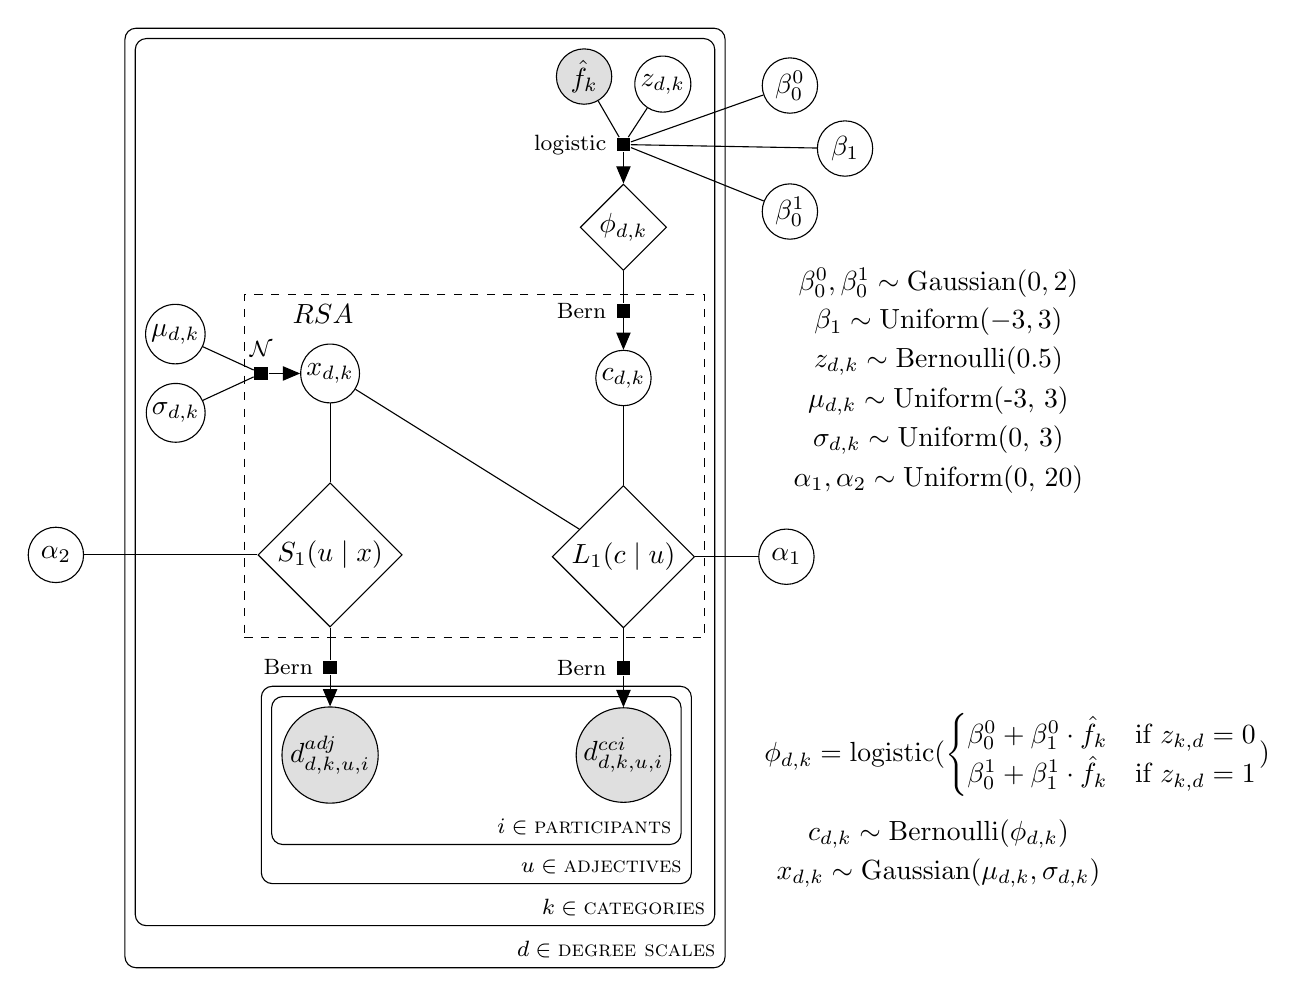
\begin{tikzpicture}


  % Y
  \node[obs]          (d-c)   {$d^{cci}_{d,k,u,i}$}; %
  \node[obs, left=2.5 of d-c]          (d-a)   {$d^{adj}_{d,k,u,i}$}; %
  \factor[above=of d-a] {da-f} {left:Bern} {} {} ; %
  \factor[above=of d-c] {dc-f} {left:Bern} {} {} ; %

  \node[det, above=of d-c] (L1) {$L_1(c \mid u)$} ; % 
  \node[det, above=of d-a] (S2) {$S_1(u \mid x)$} ; % 
  
  \node[latent, above=of S2]  (x)   {$x_{d, k}$}; %
  \node[latent, above=of L1] (c)   {$c_{d,k}$}; %
   \node[det, above= of c]  (phi) {$\phi_{d,k}$} ; %   

   \node[obs,  above=1 of phi, xshift=-0.5cm] (fhat) {$\hat{f}_k$} ; %
   \node[latent, above=0.9 of phi, xshift=0.5cm] (zi) {$z_{d, k}$} ; %
%   \edge {zi} {c}; %
%   \node[const, right=1.3 of c, yshift=1.5cm] (fshat) {$\hat{f}_s$} ; %
%   \node[latent, right=1.2 of phi, yshift=1.8cm]  (b1) {$\beta^{0}_{0}$} ; %
%   \node[latent, right=1.9 of phi, yshift=1.5cm]  (b2) {$\beta^{0}_{1}$} ; %
%   
%   \node[latent, right=1.2 of phi, yshift=0.2cm]  (b11) {$\beta^{1}_{0}$} ; %
%   \node[latent, right=1.9 of phi, yshift=0.5cm]  (b12) {$\beta^{1}_{1}$} ; %


   \node[latent, right=1.2 of phi, yshift=1.8cm]  (b1) {$\beta^{0}_{0}$} ; %   
   \node[latent, right=1.9 of phi, yshift=1cm]  (b12) {$\beta_{1}$} ; %
   \node[latent, right=1.2 of phi, yshift=0.2cm]  (b11) {$\beta^{1}_{0}$} ; %


%   \factor[above=of phi] {phi-f} {left:logistic} {fhat,b1,b2, b11, b12, zi} {phi}; %
   \factor[above=of phi] {phi-f} {left:logistic} {fhat,b1, b11, b12, zi} {phi}; %
   \factor[above=of c] {c-f} {left:Bern} {phi} {c}; %

  \node[latent, left=1.2 of x, yshift=0.5cm] (mx) {$\mu_{d, k}$} ; %
  \node[latent, left=1.2 of x, yshift=-0.5cm]  (sx) {$\sigma_{d, k}$} ; %
  \factor[left=of x] {x-f} {above:$\mathcal{N}$} {mx,sx} {x} ; %

  % sopt
   \node[latent, right=0.8cm of L1, yshift=0.0cm]         (a1)   {$\alpha_1$}; %
%   \node[latent, right=0.8cm of L1, yshift=2.5cm]         (cost)   {$cost$}; %
   \node[latent, left=2.2cm of S2]         (aa1)   {$\alpha_2$}; %
%   \node[latent, left=2.5cm of S2, yshift=-0.6cm]         (aa2)   {$\alpha^{adj}_2$}; %
 % \node[const, above=of t, xshift=-0.5cm] (at)  {$\alpha_\tau$} ; %
  % \node[const, above=of t, xshift=0.5cm]  (bt)  {$\beta_\tau$} ; %

  % Factors
%  \factor[above=of t] {t-f} {left:$\mathcal{G}$} {at,bt} {t} ; %
\factoredge {L1} {dc-f} {d-c} ; %
\factoredge {S2} {da-f} {d-a} ; %
%\factor       {W'-f}   {Multi} {} {};  %
  % Connect w and x to the dot node
  \edge[-] {c,x} {L1} ;
  \edge[-] {x} {S2} ;
%  \edge[-] {L1} {RSA} ;
%  \edge[-] {S2} {RSA} ;
%  \edge[-] {cost} {L1} ;
%  \edge[-] {cost} {S2} ;
  \edge[-] {a1} {L1} ;
%  \edge[-] {a1} {S2} ;
  \edge[-] {aa1} {S2} ;
%  \edge[-] {aa2} {S2} ;

\gate {RSAgate} {(L1)(S2)(x)(c)(x-f)(c-f)} {} ; %
\node[text width=1cm] at (-3.7,5.6) {$RSA$};
  % Plates
    \plate {dataPlate} {
     (d-c)(d-a)
  } {$i \in \textsc{participants}$} ;
  
  \plate {adjPlate} { %
    (dataPlate)
%     (S2) (L1)
  } {$u \in  \textsc{adjectives}$} ;
  
    \plate {subPlate} { %
  (adjPlate)    (dataPlate)
   (fhat) (c-f) (c)   (x)(x-f)(mx)(sx)(zi)(fhat)
    %(RSA) 
    (S2) (L1) (RSAgate)%%
  } {$k \in  \textsc{categories}$} ;
  
        \plate {degreePlate} { %
 (adjPlate)    (dataPlate)(RSAgate)(subPlate)
  (x)(x-f)(mx)(sx)(zi)(fhat)
  } {$d \in  \textsc{degree scales}$} ;
  

%    \plate {superPlate} { %
%(adjPlate)  (subPlate)(fshat)    (dataPlate)(degreePlate)
%  } {$s \in  \textsc{superordinate categories}$} ;

    
%  \plate {} {%
%    (d-c)(dc-f)(dc-f-caption) %
%    (c)(da-f)(da-f-caption) %
%    (RSA) %
%    (yx.north west)(yx.south west) %
%  } {$M$} ;




%  % Define nodes
%  \node[latent]                             (u) {$u$};
%  \node[latent, above=of u, xshift=-1.2cm] (c) {${c}$};
%  \node[latent, above=of u, xshift=1.2cm]  (x) {${x}$};
%  \node[latent, above=of c, xshift=0cm] (f) {${f}$};
%  \node[latent, above=of x, xshift=0cm] (g) {${g}$};
%
%  % Connect the nodes
%  \edge {c,x} {u} ; %
%  \edge {f} {c} ; %
%  \edge {f,g} {x} ; %

\node[] at (4,6) {$\beta^0_0, \beta^1_0 \sim \text{Gaussian}(0, 2)$};
%\node[] at (4,5.5) {$\beta^0_1, \beta^1_1 \sim \text{Uniform}(-3, 3)$};
\node[] at (4,5.5) {$\beta_1 \sim \text{Uniform}(-3, 3)$};
\node[] at (4,5) {$z_{d, k} \sim \text{Bernoulli(0.5)}$};
\node[] at (4,4.5) {$\mu_{d, k}\sim \text{Uniform(-3, 3)}$};
\node[] at (4,4) {$\sigma_{d, k}\sim \text{Uniform(0, 3)}$};
\node[] at (4,3.5) {$\alpha_1, \alpha_2 \sim \text{Uniform(0, 20)}$};

\node[] at (5,0) {$\phi_{d,k} = \text{logistic} (\begin{cases} 
	\beta^0_0 +\beta^0_1\cdot \hat{f}_k  &\mbox{if } z_{k, d} = 0 \\ 
	\beta^1_0 +\beta^1_1\cdot \hat{f}_k  &\mbox{if } z_{k, d} = 1 
	\end{cases}$)};
\node[] at (4,-1) {$c_{d,k} \sim \text{Bernoulli}(\phi_{d,k})$};
\node[] at (4,-1.5) {$x_{d,k} \sim \text{Gaussian}(\mu_{d,k}, \sigma_{d,k})$};
%(3n +1)/2 & \mbox{if } n \equiv 1 \end{cases} \pmod{2}.


\end{tikzpicture}

    \end{tabular}
  \end{center}
  \caption{\small Joint Bayesian data analytic strategy of the maximal model. Two related RSA models (an adjective endorsement model $S_1$ and the comparison class inference model $L_1$) directly predict the data from Experiments 2 \& 3 ($d^{cci}$ and $d^{adj}$), respectively. Each of these models relies upon world knowledge, which varies by the degree $d$ (e.g., height) and category $k$ (e.g., basketball players)---$P(x^{d,k})$, assumed to be Normal distributions with unknown mean $\mu^d_k$ and variance $\sigma^d_k$). The prior probability of a comparison class $c_{d,k}$ is used only in the $L_1$ model, and is assumed to be a  logistic linear function encoding a basic level bias $\beta_0$ and $\beta_1$, an effect of frequency of the noun phrase $\hat{f}_k$. Our category stimuli may be either subordinate level categories of basic-level categories determined by parameter $z_{d,k}$, which gates between using two different basic-level bias comparison class parameters. Finally, each RSA model has its own speaker optimality parameter $\alpha$.}
  \label{fig:bayesnet}
\end{figure}



%We nd combine it with a basic-level bias encoded as an intercept in a logistic linear model: $P(c) \propto \beta_0 + \beta_1 \cdot \log (\hat{f}_k)$.


%The prior distribution over comparison classes $P(c \mid k)$ reflects listeners' expectations of what comparison classes are likely to be used, given that the referent is a member of a particular subordinate category $k$.
%We simplify the full comparison class inference problem to deal with reasoning about only a specific~vs.~general class.
%This prior probability of these comparison class plausibly includes a basic-level bias \cite{rosch1975family} but could also reflect how frequently these classes are used in conversation.
%\mht{update with final model: inference about sub--basic vs. basic--super item?}


%This \emph{descriptive Bayesian approach} \cite{tauber2017} coupled with explicit models of language understanding allow us to predict and explain broader coverage data sets while still constraining flexibility by forcing models to predict more distinct data points. 

\section{Bayesian Data Analysis}


\subsection{Model details}


In the baseline model, the comparison class prior is uninformed and does not provide an \emph{a priori} preference for the Specific NP or the General NP; thus, all of the by-item variability in comparison class inferences in this model must be a function of the distributional knowledge about properties.
We assume this distributional knowledge about properties $P(x \mid k)$ (e.g., heights of basketball players) takes the form of Gaussian distributions. Since the judgments we model are binary (Expt.~2: Specific NP vs. General NP; Expt.~3: binary felicity judgments), we assign relativized units to the world knowledge distributions. We fix the General category distribution to be a unit-normal distribution and infer the parameters of the Specific category distribution. 
We put the same priors over the parameters of each Specific category distribution $k$ for each degree $d$: $\mu^d_k \sim \text{Uniform}(-3, 3)$, $\sigma^d_k \sim \text{Uniform}(0, 3)$.


For the alternative models that assign some \emph{a priori} preference the Specific or General NPs, we parameterize the comparison class prior via a logistic linear model, where a basic-level bias and an effect of usage frequency can play a part: $P(c) = \text{logistic}(\beta_0 + \beta_1 \cdot \log (\frac{\hat{f}_{specific}}{\hat{f}_{general}}) )$, where $\hat{f}_k$  represents the frequency of the comparison class  $k$ NP estimated from the Google WebGram corpus, $\beta_1$ is the sensitivity of the comparison class prior to relative frequency, and $\beta_0$ is a basic-level bias.
Our crowd-sourced stimuli generation procedure (Expt.~1) presents interesting challenges and opportunities in this analysis. 
\emph{A priori}, we do not know if the NPs we use to introduce the referents (Referent NPs; those generated by participants in Expt.~1) are basic-level categories or subordinate level categories, and hence, whether the more general comparison class would correspond to a superordinate-level category or a basic-level category.
A basic-level bias could plausibly operate differently for a subordinate~vs.~basic-level inference than for a basic~vs.~superordinate level inference. 
Specifically, superordinate comparison classes might be the most implausible, because superordinate categories are more heterogenous in comparison to basic-level or subordinate-level categories.
Thus, we endow our data-analytic model with two regression coefficient parameters corresponding to the intercept term (i.e., the basic-level bias term), and introduce a Bernoulli random variable $z$ for each NP to indicate whether it is a subordinate-level term or basic-level term (Figure \ref{fig:bayesnet}).
The alternative models that do not have both basic-level bias terms or frequency effect terms follow the same parameterization with the parameters of the various lesioned components set to 0. %\footnote{
%	The reader may wonder why we introduce a Bernoulli variable for each NP rather than for each set of 3 NPs (e.g., \emph{basketball players}, \emph{soccer players}, \emph{gymnasts}~vs.~\emph{people}) since that is the format in which we elicited our NPs from participants. We noticed that not all of our item sets were consistent in how salient a common \emph{general} category would be, possibly due to typicality effects (e.g., marshmallows, chocolate, and jolly ranchers are not equally good examples of the general category \emph{candy}).  In addition, since we do not introduce participants to our General NPs (e.g., \emph{people}), it is plausible that different General NPs come to mind given different Specific NPs in the same item set. 
%}

%The RSA listener (Eq. \ref{eq:L1a}) and speaker (Eq. \ref{eq:S2}) models make quantitative predictions about comparison class interpretation and adjective endorsement, respectively.
We construct data-analytic models with both the comparison class inference and adjective endorsement RSA components as sub-models that make quantitative predictions about the data from both of these experiments (Figure~\ref{fig:bayesnet}).
The inference and endorsement sub-models share their prior world knowledge $P(x \mid k)$ (e.g., heights of basketball players), which we infer from both data sets.
The comparison class prior $P(c \mid k)$ is parameterized by logistic function, which can encode a basic-level bias and an effect of corpus frequency, depending on the model, with the following parameters on the regression coefficients:  $\beta_0 \sim \text{Gaussian}(0, 2)$, $\beta_1 \sim \text{Uniform}(-3, 3)$. 
Each RSA model has an additional speaker optimality parameter $\alpha_{i}$ which determines the degree to which speakers are assumed to be informative and which is not of direct theoretical interest.
We use priors consistent with the previous literature: $\alpha_i \sim \text{Uniform}(0, 20)$.
We ran four different models, corresponding to the different ways of parameterizing the comparison class prior: (1) flat prior model (assumes the comparison class prior is always 50/50 between specific and general class); (2) intercept only model (assumes a basic-level bias), (3) slope only model (assumes an effect of corpus frequency, but no basic-level bias), (4) slope and intercept.
We implemented the RSA and Bayesian data analysis models in the probabilistic programming language WebPPL \cite{dippl} and performed inference by running 3 MCMC chains with 450,000 iterations each, discarding the first 150,000 for burn-in. 
Convergence was checked through visual inspection of the different chains to ensure similar conclusions would be drawn from each chain independently. 

%The comparison class inference model has one speaker optimality: $\alpha^\text{1}_{1}$.
%The adjective endorsement model has two speaker optimality parameters: 
%$\{\alpha^\text{2}_{1}, \alpha^\text{2}_{2}\}$.



\subsection{Model results}

We examined the posterior distributions over parameters and posterior predictive distributions separately by chain to confirm that the model results were consistent across runs of MCMC chains, which they were. 
Our BDA model returns posterior distributions over the parameters of the RSA models, governing world knowledge, the comparison class prior, and the speaker optimality parameters. We first determine which parameterization of the comparison class prior (flat, basic-level bias, frequency, basic-level bias and frequency) is the best for our comparison class inference RSA model to predict the comparison class inference data. 
We do so by examining the model's posterior predictive distribution over comparison class inference choices.
The posterior predictive distribution marginalizes over the inferred values of the parameters to show what data the model would expect to see, given the parameters it has learned from the data. 
Posterior predictive checks are an important step in model validation and provide a window into the model's strengths and shortcomings. 
%and (2) comparing the marginal likelihood of the data under each model to compute a Bayes Factor (BF) as a measure of formal model comparison. BFs quantify how well the model predicts the data, averaging over the prior distribution over parameters; by taking the average over the model's prior distribution over parameters, the measure explicitly takes into account model complexity because higher complexity models have wider prior distributions over the parameter \cite{lee2014bayesian}.




All models do a good job at accommodating the Adjective Endorsement data (Figure \ref{fig:scatters}, bottom row).
The BDA models adjust the parameters of the world knowledge priors used in RSA in such a way as to make the adjectives felicitous for the categories in question; in this way, the adjective endorsement task (Expt.~3) serves as a norming data set. 
This result is a good sanity check; it shows that the adjective endorsement data is directly constraining the parameters of the world knowledge priors. 
We see this reflected in the imputed world knowledge priors, which reflect intuitively accurate general expectations about the categories (Figure \ref{fig:worldPriors}). 

%\begin{figure}[t!]
%\centering
%\includegraphics[width=\textwidth]{figs/reconstructed_world_priors.pdf}
%%{\centering \includegraphics{figs/bars_adj_finalExpt_pilot_byItem} }
%\caption{xxx.}\label{fig:worldPriors}
%\end{figure}


\begin{figure}[t!]
    \centering
    \subfigure[Imputed prior distributions over degrees for 8 of the 90 item sets. These distributions were generated from the Maximum A-Posteriori parameter values inferred by conditioning on the Comparison Class Inference (Expt.~2) and Adjective Endorsement (Expt.~3)  data sets. See Figure \ref{fig:bayesnet} for full data-analytic model.]{\label{fig:worldPriors}\includegraphics[width=\textwidth]{figs/reconstructed_world_priors.pdf}} \\
    \subfigure[Human data and model predictions for items with small residuals (left 4) and largest residuals (right 4). ]{\label{fig:residuals}\includegraphics[width=\textwidth]{figs/bars_ccinfOnly_finalExpt_byNP_topResdiuals_intercept_slope_300k.pdf}}
    \caption{Quantitative modeling results.}
\end{figure}


%\begin{figure}[t!]
%\centering
%\includegraphics[width=\textwidth]{figs/bars_ccinfOnly_finalExpt_byNP_topResdiuals_intercept_slope_300k.pdf}
%%{\centering \includegraphics{figs/bars_adj_finalExpt_pilot_byItem} }
%\caption{Human data and model predictions for items with small residuals (left 4) and largest residuals (right 4).}\label{fig:residuals}
%\end{figure}


The predictions of the different model variants come apart for the Comparison Class Inference data (Expt.~2; Figure \ref{fig:scatters}). 
The baseline Flat Prior model predicts variability in comparison class inferences only as a function of world knowledge about the properties, assuming all comparison classes are equally likely \emph{a priori}; this model explains roughly 17\% of the variance.
The Frequency effect model assumes NPs with higher usage frequency will more likely be used as comparison classes and is able to explain roughly 52\% of the variance.
The Basic-level bias model explains roughly 73\% of the variance by assuming that basic-level comparison classes may be more likely \emph{a priori} and segregates the set of stimuli into those for which it believes the basic-level category is the Specific NP or those for which the basic-level category is the unmentioned, more general category. 
Finally, the maximally parameterized \emph{Basic-level and Frequency effect} -- a combination of the two alternative models -- gives rise to the best model predictions in terms of variance explained (78\%) and mean squared error (Table \ref{tab:r2bf}), suggesting that the structure of the comparison class reflects both a basic-level bias and an effect of the frequency of the NP, in addition to other possible factors. 



%The parameterization of the comparison class prior does not directly affect the model's predictions for the Adjective Endorsement (Expt.~3) data; these predictions are purely a function of the RSA model (see Supplement) and the distributional world knowledge used for both experiments (e.g., the distributions of heights for people). Thus, it is no surprise that all model variants do a good job at explaining the Adjective Endorsement data, and it is a good sanity check that the adjective endorsement RSA model is of the right form to accommodate the Adjective Endorsement data. 
%Our full model does a quite good job at accounting for the gradability of these inferences ($r = 0.88; r^2 = 0.77$)

\begin{center}
  \begin{table}[h]
    \centering
    \pgfplotstabletypeset[sci zerofill,
    col sep = comma,
    every head row/.style={before row = \toprule, after row = \midrule},
    every last row/.style={after row = \bottomrule},
    columns/model_variant/.style={string type, column name={Model}, column type = l},
    columns/subordinateCC_r2/.style={string type, column name={$r^2$ Expt.~2}, column type = l,  sci sep align, precision=3},
   columns/subordinateCC_mse/.style={fixed, column name={$MSE$ Expt.~2}, column type = l, dec sep align, precision=4},
    columns/adjEndorse_r2/.style={string type, column name={$r^2$ Expt.~3}, column type = l, sci sep align, precision=3},
     columns/adjEndorse_mse/.style={fixed, column name={$MSE$ Expt.~3}, column type = l, dec sep align, precision=4}]{csv_data_4_tex/mse_r2_table.csv}\caption{Model evaluation results. Full basic-level and frequency model exhibits the best fit to both data sets in terms of variance explained $(r^2)$ and mean squared error (MSE).}
    \label{tab:r2bf}
  \end{table}
\end{center}




To gain further insight into the comparison class inference results, we examine the full model's posterior distribution over parameters.
We start with the global parameters. As a sanity check, the speaker optimality parameters for each task were inferred to be values for which listeners assuming a rational speaker and consistent with the prior literature on RSA models --- means and 95\% Bayesian credible intervals: $\alpha_1 =  \hdiresults{model_params_cis.csv}{byItem-intercept_single-slope_speakerOptimality_subordinateCC_NA}$, $\alpha_2 =  \hdiresults{model_params_cis.csv}{byItem-intercept_single-slope_speakerOptimality_adjEndorse_NA}$.
We also find a positive effect of frequency of the noun phrase -- $\beta_1 = \hdiresults{model_params_cis.csv}{byItem-intercept_single-slope_beta_frequency_basic_super}$.

The full model infers on a by-item basis whether the basic-level category is the supplied NP or whether the basic-level category is an unmentioned, more superordinate category, because we expect the basic-level bias to operate differently for these different regimes of items.
As expected, the comparison class prior NPs that were categorized as basic-level categories strongly favored those mentioned categories -- $\beta^1_0 = \hdiresults{model_params_cis.csv}{byItem-intercept_single-slope_beta_intercept_basic_super}$.
For NPs that were categorized as subordinate categories (i.e., the basic-level category was an unmentioned, more superordinate category), the comparison class prior showed no appreciable basic-level bias -- $\beta^0_0 = \hdiresults{model_params_cis.csv}{byItem-intercept_single-slope_beta_intercept_sub_basic}$.
From these parameters values, we can compute the overall imputed prior probabilities of subordinate, basic, and superordinate comparison classes (assuming a constant effect of usage frequency), which reflect the finding that basic and subordinate comparison classes are highly accessible and superordinate comparison classes less so (Figure \ref{fig:parameters}).
%and a positive effect of frequency of the noun phrase -- $\beta^0_1 = \hdiresults{model_params_cis.csv}{byItem-intercept_single-slope_beta_frequency_sub_basic}$.



\begin{figure}[t]
\centering
\includegraphics[width=0.7\textwidth]{figs/model_comparisonClassPriorParameters.pdf}
\caption{Imputed distributions over the prior probabilities of comparison classes at different levels of abstraction. Basic- and subordinate-level categories comprise \emph{a priori} likely comparison classes, while superordinate categories are less likely to serve as comparison classes.}\label{fig:parameters}
\end{figure}

Though our fully parameterized model does the best job at accounting for the variability in comparison class inferences, the data set exhibits even more variability than our model can account for. Figure \ref{fig:residuals} shows the four item sets with largest mean model residuals (as well as the four item sets with smallest mean model residuals). 




\section{Bayesian Data Analysis}

The model's quantitative predictions can be generated by explicitly specifying the interlocutors' relevant prior knowledge (e.g., beliefs about temperatures). 
The current methodological standard is to measure prior beliefs empirically by creating tasks for participants to estimate quantities or give likelihood judgments \cite{Franke2016}. 
We pursue a different methodology. 
The RSA model captures a productive fragment of natural language; thus, it makes predictions about a related natural language task.
Critically, we can use the model to predict natural language judgments that require the \emph{same prior knowledge} as in Expt. 1 and use Bayesian data analysis to jointly infer the shared priors. 
This approach harnesses the productivity of language into experiment design and allows us to reconstruct priors without having participants engage in challenging numerical estimation tasks.

\subsection{Overview of data analytic approach}

The behavioral experiment bore out our two qualitative predictions
derived from the comparison class inference model. The model is a
quantitative model, however, and can make quantitative predictions
concerning the strength of comparison class inferences. Indeed, we
observe substantial variability in the predicted inferences both within-
and across- scales. Here we test whether the observed variability in
inferences can be accounted for by the constructs posited in our model.
We describe the two relevant constructs---the comparison class prior
\(P(c)\) and the degree priors \(P(x \mid c)\)---before outlining our
Bayesian data analytic strategy.

\subsubsection{Comparison class prior}

\(P(c)\) reflects listeners' expectations of what classes are likely to be discussed. As a proxy for comparison class usage frequency, we use empirical frequency \(\hat{f}\) estimated from the Google WebGram corpus\footnote{Corpus accessed via
\url{https://corpora.linguistik.uni-erlangen.de/cgi-bin/demos/Web1T5/Web1T5_freq.perl}. 
Due to potential polysemy and idiosyncracies of our experimental
  materials (Table 1), we made the following substitutions when querying
  the database for empirical frequency: produce $\rightarrow$
  ``fruits and vegetables''; things you watch online
  $\rightarrow$ ``online videos''; days in \{season\}
  $\rightarrow$ ``\{season\} days''; dishwashers $\rightarrow$
  ``dishwashing machines''; videos of cute animals $\rightarrow$
  ``animal videos''.}, and scale it by a free parameter $\beta$ such that $P(c) \propto \exp{(\beta \cdot \log \hat{f})}$.

\subsubsection{Degree priors (World knowledge)}

Only the relative values for \(P(x \mid c_{sub})\) and \(P(x \mid c_{super})\) affect model predictions. 
Hence we fix each superordinate distribution to be a standard normal distribution \(P(x \mid c_{super}) = \mathcal{N}(0, 1)\) and the subordinate priors to also be Gaussian distributions \(P(x \mid c_{sub}) = \mathcal{N}(\mu_{sub}, \sigma_{sub})\); the subordinate priors thus have standardized units.

Specifying the relevant prior knowledge yields two free parameters per subordinate class. We put priors over these parameters and infer their likely values using Bayesian data analysis. The data from the comparison class inference experiment would be insufficient, however, to reliably estimate all of the parameters of this data analytic model. To alleviate this, we use the same RSA model to predict additional data about related language used in the same domains. Specifically, we gather judgments about adjectives when the comparison class is explicit (\(n = 100\)): whether or not an adjective would apply to a subordinate member explicitly relative to the superordinate category (e.g., Is a day in winter warm relative to other days of the year?).\footnote{The judgments in this experiment were consistent with the \emph{a priori} ordering of the subordinate categories on the degree scale (e.g., a day in winter is likely to be cold for the year).}

To model this adjective endorsement data, we remove comparison class uncertainty by setting \(P(c_{super}) = 1\), since the sentence being endorsed include an explicit comparison to the superordinate class. We model sentence endorsement using a pragmatic speaker (following Qing \&Franke, 2014a; Tessler \& Goodman, 2016a, 2016b): \vspace{-0.5cm}
\begin{equation}
S_{2}(u \mid c_{sub}) \propto \exp{(\alpha_2 \cdot {\mathbb E}_{x\sim P_{c_{sub}}} \ln{L_1(x \mid u)})} \label{eq:S2a}
\end{equation} 

\noindent Note that $L_1(x \mid u)$ is defined from Eq. \ref{eq:L1a} by marginalization.

Eqs. \ref{eq:L1a} and \ref{eq:S2} define models for the comparison class inference task and adjective endorsement task, respectively, and depend on the same background knowledge \(P(x\mid c)\). We can thus use data from both experiments to jointly reconstruct the shared prior knowledge and generate predictions for the two data sets.

\section{Full model analysis and results}

The RSA listener (Eq. \ref{eq:L1a}) and speaker (Eq. \ref{eq:S2}) models make quantitative predictions about comparison class interpretation and adjective endorsement, respectively. We construct a single data-analytic model with each of these RSA components as sub-models in order to make quantitative predictions about the data from both of our experiments.

The listener and speaker sub-models share their prior world knowledge \(P(x \mid c)\) (e.g., temperatures in winter), described in the \textbf{Degree Priors} section. We put the same priors over the parameters of each subordinate distribution:
\(\mu \sim \text{Uniform}(-3, 3)\), \(\sigma \sim \text{Uniform}(0, 5)\), since they have standardized units. The comparison class prior \(P(c)\) in Eq. \ref{eq:L1a} scales the empirical frequency \(\hat{f}\) by a free parameter, which we give the following prior: \(\beta \sim \text{Uniform}(0, 3)\).

The full model has three additional parameters not of direct theoretical interest: the speaker optimality parameters \(\alpha^\text{expt}_{i}\), which can vary across the two tasks. The pragmatic listener \(L_1\) model (Eq. \ref{eq:L1a}) has one speaker optimality: \(\alpha^\text{1}_{1}\). The pragmatic speaker \(S_2\) model (Eq. \ref{eq:S2}) has two speaker optimality parameters: \(\{\alpha^\text{2}_{1}, \alpha^\text{2}_{2}\}\). We use priors consistent with the previous literature: \(\alpha_1 \sim \text{Uniform}(0, 20)\), \(\alpha_2 \sim \text{Uniform}(0, 5)\)

We implemented the RSA and Bayesian data analysis models in the probabilistic programming language WebPPL (Goodman \& Stuhlmuller, 2014). To learn about the credible values of the parameters, we collected 2 chains of 50k iterations (after 25k burn-in) using an incrementalized version of MCMC (Ritchie, Stuhlmuller, \& Goodman, 2016).

\subsubsection{Results}

The full model's posterior over the RSA and data-analytic parameters were consistent with prior literature and intuition. The maximum a-posteriori (MAP) estimate and 95\% highest probability density (HPD) intervals for model parameters specific to the \(L_1\) model used for comparison class inference were \(\alpha^{1}_{1} = 1.60 [1.10, 2.50]\),
\(\beta = 0.13 [0.11, 0.19]\). Model parameters specific to the \(S_2\) model used for adjective endorsement:
\(\alpha^{2}_{1} = 3.50 [0.60, 13.20]\), \(\alpha^{2}_{2} = 3.20 [2.60, 3.80]\). The inferred distributions corresponding to subordinate class priors were consistent with the \emph{a priori} ordering of these subordinate classes (low, medium, high) used in these tasks (Figure \ref{fig:modelParameters} top).

Finally, the full model's posterior predictive distribution does an excellent job at capturing the quantitative variability in comparison class inferences: \(r^2(30) = 0.96\), and adjective endorsements: \(r^2(30) = 0.98\) (Figure \ref{fig:posteriorPredictiveScatters}). Because of the overall preference for the subordinate comparison class, many of the data points are distributed above 0.5. Even for these fine-grained differences, the model does a good job at explaining the quantitative variability in participants' data (Figure \ref{fig:posteriorPredictiveScatters} right). Thus, the variability in comparison class inferences we observe in our behavioral data can be accounted for the constructs posited in our model (namely, the comparison class prior and degree priors).

\subsection{Fully Bayesian analysis of Bayesian language
models}

The second contribution of this paper is a novel data-analytic approach,
where prior knowledge used in the Bayesian language model is
reconstructed from converging evidence gathered from a related language
experiment, also explicitly modeled using a language understanding
model. In previous work, we have attempted to measure prior knowledge by
decomposing what would be a single, implicitly multilayered, numerical
estimation question into multiple simpler questions. Then, we construct
a Bayesian data analytic model to back out the prior knowledge (Tessler
\& Goodman, 2016a, 2016b). We extend this approach by using the same
core RSA model to model behavior across two language experiments. The
major feature of this method is that participants respond only to
simple, natural language questions rather than estimating numerical
quantities for which complicated linking functions must be designed
(e.g., Franke et al., 2016). The fully Bayesian language approach we
pioneer here also provides a further constraint on the language model,
which must predict data from two similar but distinct language
experiments. The productivity of natural language can thus be harnessed
to productively design experiments that further constrain and test
computational models of language and cognition.


\newpage


\bibliographystyle{apacite}

%\setlength{\bibleftmargin}{.125in}
%\setlength{\bibindent}{-\bibleftmargin}

\bibliography{comparison-class}

\end{document}
